\documentclass{article}

\usepackage{fullpage}
\usepackage{color}
\usepackage{amsmath}
\usepackage{url}
\usepackage{verbatim}
\usepackage{graphicx}
\usepackage{parskip}
\usepackage{amssymb}
\usepackage{nicefrac}
\usepackage{listings} % For displaying code
\usepackage{algorithm2e} % pseudo-code

% Answers
\def\ans#1{\par\gre{Answer: #1}}

% Colors
\definecolor{blu}{rgb}{0,0,1}
\def\blu#1{{\color{blu}#1}}
\definecolor{gre}{rgb}{0,.5,0}
\def\gre#1{{\color{gre}#1}}
\definecolor{red}{rgb}{1,0,0}
\def\red#1{{\color{red}#1}}
\def\norm#1{\|#1\|}

% Math
\def\R{\mathbb{R}}
\def\argmax{\mathop{\rm arg\,max}}
\def\argmin{\mathop{\rm arg\,min}}
\newcommand{\mat}[1]{\begin{bmatrix}#1\end{bmatrix}}
\newcommand{\alignStar}[1]{\begin{align*}#1\end{align*}}
\def\half{\frac 1 2}

% LaTeX
\newcommand{\fig}[2]{\includegraphics[width=#1\textwidth]{a3f/#2}}
\newcommand{\centerfig}[2]{\begin{center}\includegraphics[width=#1\textwidth]{a3f/#2}\end{center}}
\newcommand{\matCode}[1]{\lstinputlisting[language=Matlab]{a3f/#1.m}}
\def\items#1{\begin{itemize}#1\end{itemize}}
\def\enum#1{\begin{enumerate}#1\end{enumerate}}


\begin{document}

\title{CPSC 340 Assignment 3 (due Friday October 11 at 11:55pm)}
\author{}
\date{}
\maketitle
\vspace{-4em}

On this assignment, we are only going to allow a \blu{maximum of 1 ``late class''} to be used. This is because the midterm is on October 17th, and we want to give you more than 1 day to look at the solutions before the actual exam.

\section{More Unsupervised Learning}

 \subsection{$k$-Medians}
 
 The data in \emph{clusterData2.jl} is the exact same as \emph{clusterData.jl} from a previous question, except it has 4 outliers that are far away from the data.
 
 \blu{\enum{
 \item Using the \emph{clustering2Dplot} function, output the clustering obtained by running k-means 50 times (with $k=4$) on \emph{clusterData2.mat} and taking the one with the lowest error. Are you satisfied with the result?  \ans{ 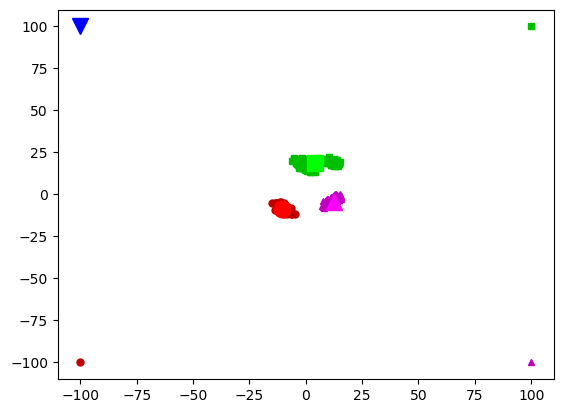
\includegraphics[width=10cm]{q1Class.png}  No, the algorithm have detected 3 Classed in the middle, but in the previous assignments, it should ideally identify 4 classed in the middle. But in this condition, an outlier have taken away one of the class.}
 \item What values of $k$ might be chosen by the elbow method for this dataset? \ans{3}
 \item Implement the $k$-\emph{medians} algorithm, which assigns examples to the nearest $w_c$ in the L1-norm and then updates the $w_c$ by setting them to the ``median" of the points assigned to the cluster (we define the $d$-dimensional median as the concatenation of the medians along each dimension). For this algorithm it makes sense to use the L1-norm version of the error (where $y_i$ now represents the closest median in the L1-norm),
\[
f(w_1,w_2,\dots,w_k,y_1,y_2,\dots,y_n) = \sum_{i=1}^n \norm{x_i - w_{y_i}}_1 = \sum_{i=1}^n \sum_{j=1}^d |x_{ij} - w_{y_ij}|,
\] 
 Hand in your code and plot obtained by taking the clustering with the lowest L1-norm after using  50 random initializations for $k = 4$.
\ans{\\Code on next page. \\ 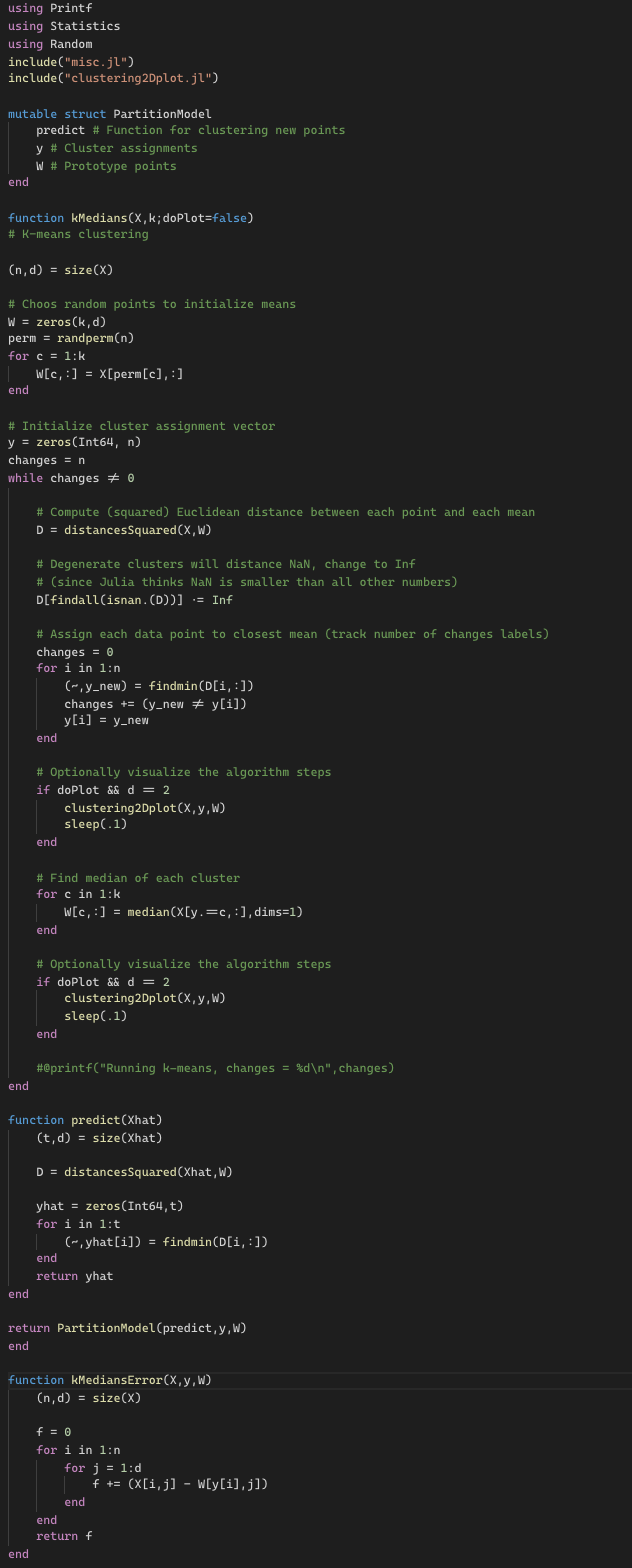
\includegraphics[width = 10cm]{q13Code.png} \\ 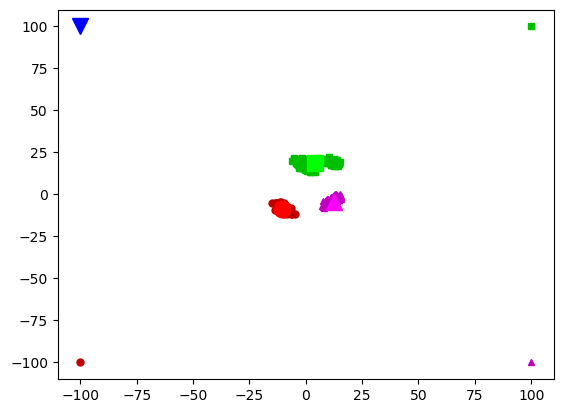
\includegraphics[width=10cm]{q1Class.png}}
 \item What value of $k$ would be chosen by the elbow method if you k-medians and the L1-norm? Are you satisfied with this result?
\ans{3, yes}
 }}



\subsection{Density-Based Clustering}

If you run the function \emph{example\_dbCluster}, it will apply the basic density-based clustering algorithm to the dataset from the previous part. The final output should look like this:\\
%\fig{.49}{density}\fig{.49}{density2}\\
(The right plot is zoomed in to show the non-outlier part of the data.)
Even though we know that each object was generated from one of four clusters (and we have 4 outliers), the algorithm finds 6 clusters and does not assign some of the original non-outlier objects to any cluster. However, the clusters will change if we change the parameters of the algorithm. Find and report values for the two parameters (\emph{radius} and \emph{minPts}) such that the density-based clustering method finds:
\blu{\enum{
\item The 4 ``true" clusters. \ans{radius = 2
minPts = 2}
\item 3 clusters (merging the top two, which also seems like a reasonable interpretaition). \ans{radius = 5
minPts = 2}
\item 2 clusters. \ans{radius = 15
minPts = 2}
\item 1 cluster (consisting of the non-outlier points).\ans{radius = 20
minPts = 2}
}}





\section{Matrix Notation and Linear Regression}

\subsection{Converting to Matrix/Vector/Norm Notation}

Using our standard supervised learning notation ($X$, $y$, $w$)
express the following functions in terms of vectors, matrices, and norms (there should be no summations or maximums).
\blu{\enum{
\item $\sum_{i=1}^n  |w^Tx_i - y_i| + \lambda \sum_{j=1}^{d} |w_j|$. \ans{$w^TX - y + \lambda \|w\|_1$}
\item $\sum_{i=1}^n v_i (w^Tx_i - y_i)^2 + \sum_{j=1}^{d} \lambda_j w_j^2$. \ans{$ (w^TX-y)V \cdot (w^TX-y) + (\Lambda w) \cdot w$}
\item $\left(\max_{i \in \{1,2,\dots,n\}} |w^Tx_i - y_i|\right)^2 +  \half\sum_{j=1}^{d} \lambda_j|w_j|$.  \ans{$(\|w^Tx-y\| _{\infty})^2 + \frac{1}{2} \|\Lambda w\|_1$}
}}
You can use $V$ to denote a diagonal matrix that has the (non-negative) ``weights'' $v_i$ along the diagonal. The value $\lambda$ (the ``regularization parameter'') is a non-negative scalar. You can $\Lambda$ as a diagonal matrix that has the (non-negative) $\lambda_j$ values along the diagonal.


\subsection{Minimizing Quadratic Functions as Linear Systems}

Write finding a minimizer $w$ of the functions below as a system of linear equations (using vector/matrix notation and simplifying as much as possible). Note that all the functions below are convex  so finding a $w$ with $\nabla f(w) = 0$ is sufficient to minimize the functions (but show your work in getting to this point).

\blu{\enum{
\item $f(w) = \frac{1}{2}\norm{w-u}^2$ (projection of $v$ onto real space). \ans{ $f(w) = \frac{1}{2}\sum^d_{i=0}(w_i-u_i)^2 \\ \nabla f(w) = ((w_1-u_i), (w_2-u_i), \dots )^T$ \\ Therefore Optimized $w = u$}
\item $f(w)= \frac{1}{2}\sum_{i=1}^n v_i (w^Tx_i - y_i)^2 + \lambda w^Tu$ (weighted and tilted least squares). \ans{$ f(w) = \frac{1}{2}\sum_{i=1}^n v_i( (\sum_{j=i}^d x_i^d * w_d)-y_i )^2 + \lambda \sum_{j=1}^d {w_d}u_d \\ f(w) = \frac{1}{2}\sum_{i=1}^n v_i( \hat{y_i}-y_i )^2 + \lambda \sum_{j=1}^d {w_d}u_d = \frac{1}{2}\sum_{i=1}^n v_i (\hat{y_i}^2 + 2\hat{y_i}{y_i} + y_i^2) + \lambda \sum_{j=1}^d {w_d}u_d \\ \\\nabla f(w) = (\frac{1}{2}v_1$}
\item $f(w) = \frac{1}{2}\norm{Xw - y}^2 + \frac{\lambda}{2}\norm{w-w^0}^2$ (least squares shrunk towards non-zero $w^0$).
}}
Above we assume that $u$ and $w^0$ are $d$ by $1$ vectors, that $v$ is a $n$ by $1$ vector. You can use $V$ as a diagonal matrix containing the $v_i$ values along the diagonal.

Hint: Once you convert to vector/matrix notation, you can use the results from class to quickly compute these quantities term-wise.
As a sanity check for your derivation, make sure that your results have the right dimensions. As a sanity check, make that the dimensions match for all quantities/operations. In order to make the dimensions match you may need to introduce an identity matrix. For example, $X^TXw + \lambda w$ can be re-written as $(X^TX + \lambda I)w$.



\subsection{Convex Functions}

Recall that convex loss functions are typically easier to minimize than non-convex functions, so it's important to be able to identify whether a function is convex.

\blu{Show that the following functions are convex}:

\enum{
\item $f(w) = \alpha w^2 - \beta w + \gamma$ with $w \in \R, \alpha \geq 0, \beta \in \R, \gamma \in \R$ (1D quadratic).
\item $f(w) = w\log(w) $ with $w > 0$ (``neg-entropy'')
\item $f(w) = \norm{Xw-y}^2 + \lambda\norm{w}_1$ with $w \in \R^d, \lambda \geq 0$ (L1-regularized least squares).
\item $f(w) = \sum_{i=1}^n \log(1+\exp(-y_iw^Tx_i)) $ with $w \in \R^d$ (logistic regression).
\item $f(w) = \sum_{i=1}^n[\max\{0,|w^Tx_i - y_i|\} - \epsilon] + \frac{\lambda}{2}\norm{w}_2^2$  with $w \in \R^d, \epsilon \geq 0, \lambda \geq 0$ (support vector regression).
}

General hint: for the first two you can check that the second derivative is non-negative since they are one-dimensional. For the last 3 you'll have to use some of the results regarding how combining convex functions can yield convex functions which can be found in the lecture slides.

Hint for part 4 (logistic regression): this function may seem non-convex since it contains $\log(z)$ and $\log$ is concave, but there is a flaw in that reasoning: for example $\log(\exp(z))=z$ is convex despite containing a $\log$. To show convexity, you can reduce the problem to showing that $\log(1+\exp(z))$ is convex, which can be done by computing the second derivative. It may simplify matters to note that $\frac{\exp(z)}{1+\exp(z)} = \frac{1}{1+\exp(-z)}$.



\section{Linear and Nonlinear Regression}


If you run the script \emph{example\_nonLinear}, it will:
\enum{
\item Load a one-dimensional regression dataset.
\item Fit a least-squares linear regression model.
\item Report the training error.
\item Report the test error (on a dataset not used for training).
\item Draw a figure showing the training data and what the linear model looks like.
}
Unfortunately, this is an awful model of the data. The average squared training error on the data set is over 28000 (as is the test error), and the figure produced by the demo confirms that the predictions are usually nowhere near the training data:
%\centerfig{.5}{leastSquares}


\subsection{Linear Regresion with Bias Variable}

The y-intercept of this data is clearly not zero (it looks like it's closer to $200$), so we should expect to improve performance by adding a \emph{bias} variable, so that our model is
\[
y_i = w^Tx_i + w_0.
\]
instead of
\[
y_i = w^Tx_i.
\]
\blu{Write a new function, \emph{leastSquaresBias}, that has the same input/model/predict format as the \emph{leastSquares} function, but that adds a \emph{bias} variable $w_0$. Hand in your new function, the updated plot, and the updated training/test error.}

Hint: recall that adding a bias $w_0$ is equivalent to adding a column of ones to the matrix $X$. Don't forget that you need to do the same transformation in the \emph{predict} function.


\subsection{Linear Regression with Polynomial Basis}

Adding a bias variable improves the prediction substantially, but the model is still problematic because the target seems to be a \emph{non-linear} function of the input. Write a new function, \emph{leastSquaresBasis(x,y,p)}, that takes a data vector $x$ (i.e., assuming we only have one feature) and the polynomial order $p$. The function should perform a least squares fit based on a matrix $Z$ where each of its rows contains the values $(x_{i})^j$ for $j=0$ up to $p$. E.g., \emph{leastSquaresBasis(x,y,3)} should form the matrix
\[
Z = 
\left[\begin{array}{cccc}
1 & x_1 & (x_1)^2 & (x_1)^3\\
1 & x_2 & (x_2)^2 & (x_2)^3\\
\vdots\\
1 & x_n & (x_n)^2 & (x_N)^3\\
\end{array}
\right],
\]
and fit a least squares model based on it.
\blu{Hand in the new function, and report the training and test error for $p = 0$ through $p= 10$. Explain the effect of $p$ on the training error and on the test error.}

Note: for this question we'll assume $d=1$ (we'll discuss polynomial bases with more input features later in the course).

Hints: To keep the code simple and reduce the chance of having errors, you may want to write a new function \emph{polyBasis} that you can use for transforming both the training and testing data. 



\subsection{Manual Search for Optimal Basis}

Polynomials are a flexible class of functions, but there is structure in this data that is not well-modelled by polynomials. Try to find a nonlinear basis that gives the best performance on this dataset in terms of test error. \blu{Report the basis that you use and the training/test score that you achieve}.

Hint: the data seems to have periodic behaviour, and it's possible to obtain training and test errors below 60.

\section{Robust Regression and Gradient Descent}

The script \emph{example\_outliers} loads a one-dimensional regression dataset that has a non-trivial number of `outlier' data points. These points do not fit the general trend of the rest of the data, and pull the least squares model away from the main downward trend that most data points exhibit:
%\centerfig{.7}{outliers}




\subsection{Weighted Least Squares in One Dimension}

One of the most common variations on least squares is \emph{weighted} least squares. In this formulation, we have a weight $v_i$ for every training example. To fit the model, we minimize the weighted squared error,
\[
f(w) =  \frac{1}{2}\sum_{i=1}^n v_i(w^Tx_i - y_i)^2.
\]
In this formulation, the model focuses on making the error small for examples $i$ where $v_i$ is high. Similarly, if $v_i$ is low then the model allows a larger error.

Write a model function, \emph{weightedLeastSquares(X,y,v)}, that implements this model (note that this can be solved as a linear system).
Apply this model to the data containing outliers, setting $v_i = 1$ for the first $400$ data points and $v_i = 0.1$ for the last $100$ data points (which are the outliers). \blu{Hand in your function and the updated plot}.


\subsection{Smooth Approximation to the L1-Norm}

Unfortunately, we typically do not know the identities of the outliers. In situations where we suspect that there are outliers, but we do not know which examples are outliers, it makes sense to use a loss function that is more robust to outliers. In class, we discussed using the Huber loss,
\[
f(w) = \sum_{i=1}^n h(w^Tx_i  -y_i),
\]
where
\[
h(r_i) = 
\begin{cases}
\half r_i^2 & \text{for $|r_i| \leq \epsilon$}\\
\epsilon(|r_i| - \half \epsilon) & \text{otherwise}
\end{cases}.
\]
This is less sensitive to outliers than least squares, although it can no longer be minimized by solving a linear system.
 \blu{Derive
 the gradient $\nabla f$ of this function with respect to $w$. You should show your work but you do not have to express the final result in matrix notation.}
 Hint: you can start by computing the derivative of $h$ with respect to $r_i$ and then get the gradient using the chain rule. You can use sgn$(r_i)$ as a function that returns $1$ if $r_i$ is positive and $-1$ if it is negative.


\subsection{Robust Regression}

The function \emph{example\_gradient} is the same as \emph{example\_outlier}, except that it fits the least squares model using a \emph{gradient descent} method. You'll see that it produces the same fit as we obtained using the normal equations.

The typical input to a gradient method is a function that, given $w$, returns $f(w)$ and $\nabla f(w)$. See \emph{funObj} in the \emph{leastSquaresGradient} function for an example. Note that \emph{leastSquaresGradient} also has a numerical check that the gradient code is approximately correct, since implementing gradients is often error-prone.\footnote{Though sometimes the numerical gradient checker itself can be wrong. For a lot more on numerical differentiation you can take CPSC 303.}

An advantage of gradient-based strategies is that they are able to solve problems that do not have closed-form solutions, such as the formulation from the previous section. The function \emph{robustRegression} has most of the implementation of a gradient-based strategy for fitting the Huber regression model. The only part missing is the function and gradient calculation inside the \emph{funObj} code. \blu{Modify this function to implement the objective function and gradient based on the Huber loss (from the previous section). Hand in your code, as well as the plot obtained using this robust regression approach \red{with $\epsilon = 1$}.}

\section{Very-Short Answer Questions}



\begin{enumerate}
\item Describe a dataset with $k$ clusters where k-means cannot find the true clusters.
\item Why do we need random restarts for $k$-means but not for density-based clustering?
\item Can hierarchical clustering find non-convex clusters?
\item For each outlier detection method below, list an example method and a problem with identifying outliers using this method:
\begin{itemize}
\item Model-based outlier detection.
\item Graphical-based outlier detection.
\item Supervised outlier detection.
\end{itemize}
\item In linear regression, why do we compute the squared error $(y_i -  \hat{y}_i)^2$ and not test the equality $(y_i = \hat{y}_i)$?
\item Describe a simple 2-feature ($d=2$) case where the least squares estimate would not be unique.
\item Why do we typically add a column of $1$ values to $X$ when we do linear regression? Should we do this if we're using decision trees?
\item When should we consider using gradient descent to approximate the solution to the least squares problem instead of exactly solving it with the closed form solution? 
\item If a function is convex, what does that say about stationary points of the function? Does convexity imply that a stationary points exists?
\item For robust regression based on the L1-norm error, why can't we just set the gradient to 0 and solve a linear system? In this setting, why we would want to use a smooth approximation to the absolute value? 
\item What is the problem with having too small of a learning rate in gradient descent?
\item What is the problem with having too large of a learning rate in gradient descent?
\end{enumerate}


\section*{Project Proposal (OPTIONAL FOR 340 STUDENTS)}

For 532M students, there is a project component to the course that will be worth 20\% of your final grade. For 340 students, there is no requirement to do a project. However, 340 students have the option to do a project anyway for the possibility of obtaining a higher grade: your project grade can replace either your 2 lowest assignment scores or your midterm score (whicheve helps you more).\footnote{The course is \emph{not} graded on a curve, so 340 students are not hurt by choosing the to skip the project.}

This semester you will have the option of doing two styles of projects:
\enum{
\item \textbf{Small Projects}: These projects are done in \blu{groups of 2-3}. The final deliverable will be a \blu{6-page report that is due near the end of the exam period} (something like December 16th). It is expected that this project will be a literature survey, but research projects are also ok.
\item \textbf{Big Projects}: These projects are done in \blu{groups of approximately 5} (4 or 6 is ok if needed but I would prefer you aim for 5). The final deliverable will be a \blu{poster to be presented December 8th} from 4-7pm at a hotel downtown (probably the Fairmont Waterfront). Students from a similar class at SFU will also be presenting their posters during this time, and over 50 companies (looking to potentially hire people like you) will also be there.
}
There aren't really any restrictions on the group compositions: 340 students can work with 532M students, auditors can work with registered students, and you can combine this project with a project from another one of your classes (assuming you get the other instructor's permission, and even if not all students in the other class are registered in this class). The only combinations I really want to avoid are having students do projects with the TAs (due to the obvious conflict of interest), project groups that have no students enrolled in 340 or 532M, or projects that contain people taking no CPSC classes.

If you are in 532M, or in 340 and want to do a project, for the final part of this assignment you must a \blu{submit a project proposal} for your course project. The proposal should be a maximum of 2 pages (and 1 page or half of a page is ok if you can describe your plan concisely). The proposal should be written for the instructors and the TAs, so you don't need to introduce any ML background but you will need to introduce non-ML topics. 

\blu{You should submit this question as a group on Gradescope, separate from the other assignment questions.} 

There is quite a bit of flexibility in terms of the type of project you do, as I believe there are many ways that people can make valuable contributions to research. However, note that ultimately the final deliverable for the project will be a report/poster that emphasizes a particular ``contribution" (i.e., what doing the project has added to the world).
The reason for this, even though it's strange for some possible projects, is that this is the standard way that results are communicated to the research community.

\blu{The three mains ingredients of the project proposal are:
\begin{enumerate}
\item What problem you are focusing on.
\item What you plan to do.
\item What will be the ``contribution".
\end{enumerate}
}
Also, for the course project note that negative results (i.e., we tried something that we thought we would work in a particular setting but it didn't work) are acceptable (and often unavoidable).

If you are doing a small project, the default ``template'' for the project is the following:
\enum{
\item \textbf{Literature review}: you pick a specific topic in ML, read at least 10 papers on the topic, then write a report summarizing what has been done on the topic and what are the most promising directions of future work. In this case, the contribution would be your summary of the relationships between the existing works, and your insights about where the field is going.
}
Here are some standard ``templates'' for a big project (you also have the option of using these for small projects):
\enum{
\setcounter{enumi}{1}
\item \textbf{Application bake-off}: you pick a specific application (from your research, personal interests, or maybe from Kaggle) or a small number of related applications, and try out a bunch of techniques (e.g., random forests vs. logistic regression vs. generative models). In this case, the contribution would be showing that some methods work better than others for this specific application (or your contribution could be that everything works equally well/badly).
\item \textbf{New application}: you pick an application where people aren't using ML, and you test out whether ML methods are effective for the task. In this case, the contribution would be knowing whether ML is suitable for the task.
\item \textbf{Scaling up}: you pick a specific machine learning technique, and you try to figure out how to make it run faster or on larger datasets. In this case, the contribution would be the new technique and an evaluation of its performance, or could be a comparison of different ways to address the problem.
\item \textbf{Improving performance}: you pick a specific machine learning technique, and try to extend it in some way to improve its performance. In this case, the contribution would be the new technique and an evaluation of its performance.
\item \textbf{Generalization to new setting}: you pick a specific machine learning technique, and try to extend it to a new setting (for example, making a multi-label version of random forests).  In this case, the contribution would be the new technique and an evaluation of its performance, or could be a comparison of different ways to address the problem.
\item \textbf{Coding project}: you pick a specific method or set of methods, and build an implementation of them. In this case, the contribution could be the implementation itself or a comparison of different ways to solve the problem.
\item \textbf{Theory}: you pick a theoretical topic (like the variance of cross-validation), read what has been done about it, and try to prove a new result (usually by relaxing existing assumptions or adding new assumptions). The contribution could be a new analysis of an existing method, or why some approaches to analyzing the method will not work.
\item \textbf{Reproducibility Challenge}: you take part in the 2019 NeurIPS reproducibility challenge, where you try to reproduce the results of a recently-submitted machine learning paper. Information on the challenge is available here (watch out for the early deadline if you want to officially take part): \\\url{https://reproducibility-challenge.github.io/neurips2019}
}
The above are just suggestions, and many projects will mix several of these templates together, but if you are having trouble getting going then it's best to stick with one of the above templates. Also note that the project can focus on topics not covered in the course (like RNNs), so there is flexibility in the topic, but the topic should be closely-related to ML.

\blu{This question is mandatory but will not be formally marked: it's just a sanity check that you have at least one project idea that has an appropriate topic and scope, that you find a group early, and that you  allocate some time to thinking about the project.} 
Also, there is flexibility in the choice of project topics even after the proposal: if you want to explore different topics you can ultimately choose to do a project that is unrelated to the one in your proposal (and changing groups is ok too). If you aren't sure what to do, go bug the TAs in office hours (which is a good idea even if you are sure what you want to).



\end{document}